\section{Literature Review}
\subsection{Stewart Platform}
Parallel link manipulators have become an important area of research due to their: precision, rigidity and high-load-to-weight ratio. These manipulators find practical applications in flight simulators, precise machining and applications that require disturbance isolation. \cite{iqbal_dynamic_2008}. The Stewart platform is an example of a parallel manipulator.

A Stewart platform is a parallel manipulator that provides six-degree-of-freedom (DOF) i.e. roll, pitch, yaw, surge, sway and heave, and can be controlled in all these freedoms simultaneously. The platform consists six variable-length electro-mechanical actuators connecting a top plate to a base plate with spherical joints.

The platform is able to move in three angular directions and in three linear directions, singly or in any combination \cite{stewart1965platform}. Angular and translational motion of the top plate with
respect to the base plate is achieved by reducing or extending the actuator lengths. For the top plate to follow the desired trajectory with high frequency, there has to be proper coordination of the actuator lengths \cite{iqbal_dynamic_2008}.

Each leg of the mechanism is connected to the ground by a two-axis joint where: One of these axes is
normal to the leg and is provided with a means for control whereas, the other axis is normal to the first and is not provided with a means for control.
Each leg also has controllable means for extending its length. These control means include:
\begin{enumerate}
\item Use of hydraulic jacks.
\item Screw jacks - This gives give the advantage of
a longer stroke for a given size.
\item Rotary actuator - a hydraulic rotary actuator or an electric motor. Whereas this would reduce the number of foundation fixings, the remaining jack would still be subjected to a greater bending moment.
\item Levers - this increases the extending leg amplitude by using an articulated leg.
\item Linear co-ordinate control - this arrangement provides rigidity due to the true triangulation of
the whole system. There will be no bending moments in any of the members apart from the possibility of those due to strut eccentric loading. 
\end{enumerate}
\begin{center}
	\begin{figure}[!h]
	\centering
	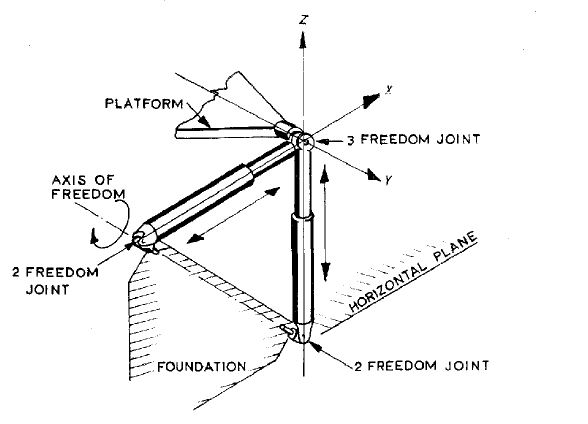
\includegraphics[width=0.6\linewidth]{Figures/Fig11}
	\caption[Linear co-ordinate control]{Linear co-ordinate control \cite{stewart1965platform}}
	\end{figure}
\end{center}

Stewart platforms that use screw jacks driven by electric motors as leg actuators have the advantage of being light and easy to control. Velocity and position control for these platforms can be done using shaft encoders and tachometers. A ball screw is used to minimize friction in a screw drive and backlash in the ball screw can be eliminated by use of double nuts preloaded with spring washers \cite{fichter1986stewart}.

The Stewart platform has drawn the interest of many researchers who have focused on solving kinematics, dynamics and control of the mechanism. Both inverse kinematic and forward kinematic methods for the Stewart platform are presented in literature
\cite{csumnu2017simulation}.

In order to control the platform in the required direction, a program involving linear or angular accelerations or a combination of both is necessary so that signals can be given to the various legs in accordance with the input requirements. The six inputs to the Stewart platform in terms of torque are calculated by the controller and the outputs of the Stewart platform are the upper plate's angular and translational positions sensed by highly precise sensors or estimated by the motor's encoders \cite{iqbal_dynamic_2008}.

Further, as concerns the control aspect, in recent years many researchers have worked on robust controllers for the Stewart platform. Some of these works include:
\begin{enumerate}
\item A Lyapunov based approach for designing robust PD controller was proposed in presence of uncertainties 
\cite{kang1996robust}.
\item The model based sliding mode control with perturbation 
\cite{kang1996robust}.
\item Robust tracking control design in the presence of time varying
uncertainties 
\cite{kim1998high}.
\item Tracking errors drive to zero asymptotically with help of sliding mode
controller design 
\cite{huang2004sliding}.
\item A simple way to calculate control law using sliding-mode technique 
\cite{iqbal2006direct}.
\end{enumerate}

\subsubsection{Wind Tunnel}
A wind tunnel is a large tube with air moving inside. This movement of air is usually done by powerful fans. 

The first wind tunnel was built by Francis Wenham in 1871. However, it was the Wright Brothers who were the first to show the value of the wind tunnel in aerodynamic design with their 1902 wind tunnel.  The Wright Brothers’ wind tunnel was largely made of wood, with a glass window on the top to look down through and see the force balance, from which the
lift and drag forces could be read. The wind tunnel was powered by a fan driven off a natural gas fueled engine. Their tunnel was square of 16" by 16"(about 407mm by 407mm), and 6 foot long (about 1829mm), with a maximum test speed of 35 mph (about 56 km/h).
\begin{center}
	\begin{figure}[!h]
	\centering
	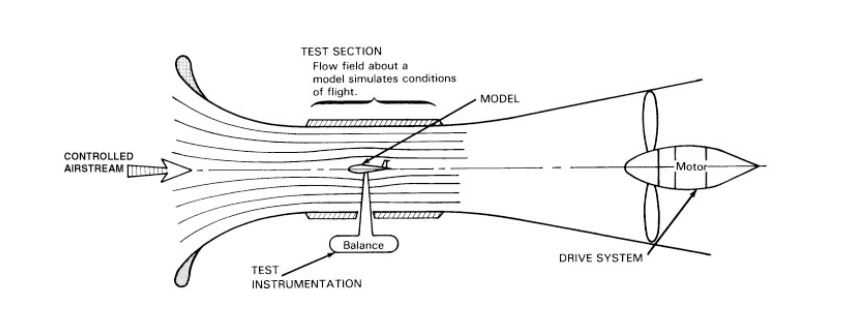
\includegraphics[width=0.75\linewidth]{Figures/Fig2}
	\caption[A Typical Wind Tunnel]{Diagram of a typical wind tunnel \cite{morris_force_2010}}
	\end{figure}
\end{center}

Later in the early 20th century in Europe, the main users of wind tunnels were Gustave Eiffel in France and Ludwig Prandtl in Germany. Prandtl built the first closed circuit wind tunnel in 1908. Closed circuit wind tunnels are characterized by the recirculation of the airflow with very minimal exchange with the exterior. Open circuit wind tunnels on the other hand, have an airflow that follows a straight path and flows to the contracted zone where the test section is located and then passes through a diffuser, a fan section and an exhaust.

By the 1940’s supersonic wind tunnels were in use. In 1972 a cryogenic wind tunnel was built at NASA Langley by injecting liquid nitrogen into the wind tunnel to cool the gas. This lowered the viscosity and increased the Reynolds number, and this tunnel had the capability to match Reynolds and Mach numbers simultaneously up to Mach 1.2
\cite{fernandes_design_nodate}.

Today the largest wind tunnel in the world is the National Full-Scale Aerodynamics Complex at NASA's Ames Research Center, which has a test section of cross-section 80 ft by 100 ft (24 m x 31 m). The types of instruments in common use in wind tunnels include boundary layer rakes, tufts, pitot tubes, pressure sensitive paint, smoke, and static pressure taps \cite{morris_force_2010}.
\begin{center}
\begin{figure}[!h]
	\centering
	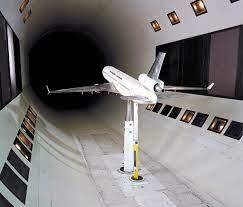
\includegraphics{Figures/Fig3}
	\caption[NASA Wind Tunnels]{NASA wind tunnels used to test new airplane designs \cite{NASA}}
\end{figure}
\end{center}

NASA uses wind tunnels to test scale models of aircraft and spacecraft. Wind tunnels help NASA to test ideas of making airplanes better and safer. They are also used to help engineers in designing spacecraft that will work in other planets such as mars - the wind tunnel can be used to simulate objects in an atmosphere that's thinner than ours e.g. an atmosphere that's exactly like the Martian atmosphere. NASA has wind tunnels of different types and sizes. Some are low-speed wind tunnels, others are hypersonic i.e. they are made to carry out tests at 4,000 mph (6437 kph) \cite{NASA}.
\begin{center}
     %&\vspace*{-4.0cm}
    \begin{figure}[!h]
\centering
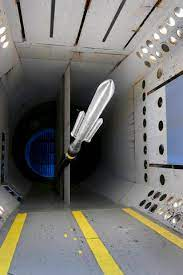
\includegraphics{Figures/Fig4}
\caption[NASA Wind tunnel - space application]{NASA wind tunnels used to test the design of heavy-lift rocket \cite{NASA}}
\end{figure}
\end{center}
\subsection{Force Balances}
For wind tunnel applications, the wind axes is used as the reference frame. Where, X axis points to the accelerated air; Z axis points downward and; Y axis points to the right in the direction of the wind. In the reference frame above, lift is in the negative z-direction, drag in the negative x-direction and, side force in the negative y-direction.

Moment components on the x,y,z axes are rolling moment, pitching moment and yawing moment respectively. A three-component force balance can be considered to measure the lift, drag and pitch (angle of attack).

Force balances can be external or internal. In external force balances the test section lies outside of the wind tunnel test section, whereas in internal force balances the balance is inside the model itself connecting the model to the support structure.

Several different types of external force balances are available for wind tunnel use
\cite{morris_force_2010}:
\begin{enumerate}
\item Wire
\item Platform
\item Yoke
\item Pyramidal
\end{enumerate}
\begin{center}
	\begin{figure}[!h]
	\centering
	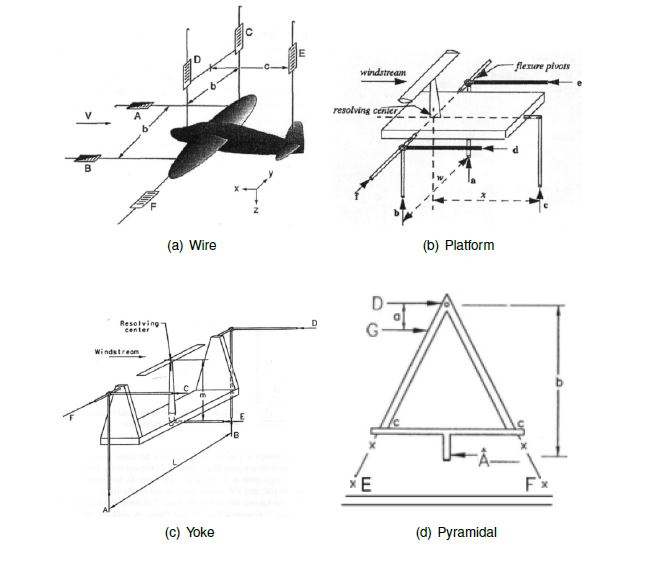
\includegraphics{Figures/Fig6}
	\caption[External Force balances]{Typical configurations for external force balances \cite{ferreira2015design}}
	\end{figure}
\end{center}
In the wire balance, the model under testing is suspended by wires each connected to an extensometer (a sensor that produces an electrical output when submitted to a load and deforms). The shortcoming of the wire balance is the large tare drag caused by the wires which is difficult to quantify. They are also not robust nor versatile enough compared with the other alternatives. 

The platform balance is relatively easy to construct, assemble and instrument. However, for this balance, forces and torques are coupled and the balance resolving center does not coincide with the center of the tunnel.
 
In the yoke balance configuration, forces and torques are coupled and the balance resolving center coincides with the center of the tunnel. This configuration, however, presents some structural deflections due to the large span of the measuring and support arms.

The pyramidal balance configuration is a further improvement of the yoke balance in order to overcome the shortcomings of the other balances. It is capable of measuring six components of forces and
torques separately and without coupling,provided that the balance is well assembled and calibrated.

The different kinds of internal balances can be made based on:
\begin{enumerate}
\item The type of transducer i.e. strain gauge or piezoelectric balance.
\item Shape i.e. box balance and sting balance
\end{enumerate} 
\begin{center}
	\begin{figure}[!h]
	\centering
	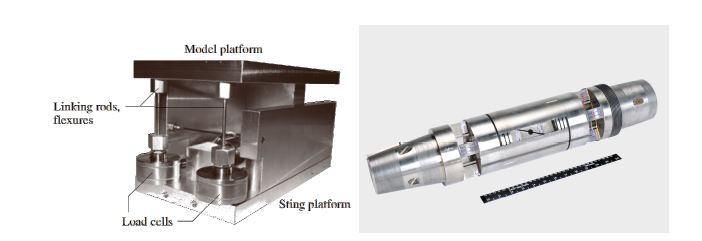
\includegraphics{Figures/Fig7}
	\caption[Internal force balances]{Typical configurations for internal force balances. \textit{Left to right:} Box balance and sting balance.}
	\end{figure}
\end{center}
The box balance presents a cubic shape and can either be made of a solid piece of material or from assembled parts. In this configuation, the loads are transferred from the top to the bottom. The sting balance presents a cylindrical shape and the loads are transferred from one end to the other in the longitudinal direction. It can be used to measure forces or torques.

The advantage of internal force balances is that they minimize the interference caused by the supporting bars in the flow.
\subsection{Sensors}
\subsubsection{Load Sensors}
Several methods can be used to measure forces and torques in a force balance. These methods can be generally grouped into two:
\begin{enumerate}
\item Hydraulic measuring techniques.
\item Electric measurement techniques.
\end{enumerate}
Electric measurement techniques are preferred for Force balance applications. One such electric measurement device is the strain gauge. A strain gauge is an electromechanical device whose electrical resistance changes linearly with the strain in the component.

Metal foil strain gauges are widely used. This type of strain gauge provide more precise strain values than wire strain gauges. However, since the relative changes on electric resistance of the strain gauge are so small, it is necessary to develop an effective method to measure them because each strain gauge would require extremely accurate signal measurements. The solution is to have a set of strain gauges coupled in order to minimize the required accuracy, forming a force transducer i.e. the \textit{Wheatstone bridge}.
\begin{center}
		\begin{figure}[!h]
		\centering
		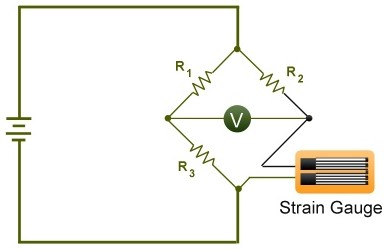
\includegraphics[width=0.6\linewidth]{Figures/Fig9}
		\caption[Wheatstone Bridge Circuit]{Wheatstone Bridge Circuit \cite{ferreira2015design}}
		\end{figure}
\end{center}
Load cells can also be used to measure the drag and lift forces.
\subsubsection{Attitude Sensor}
It is important to define the desired aerodynamic angles and to guarantee that they are measured accurately in relation to the air stream. One such angle is the angle of attack (\textalpha) shown in Figure 2.4. For this reason, specific devices that provide the attitude measurement should be implemented in order to improve the precision of the results.

Angle of attack (\textalpha)- angle measured between the longitudinal axis of the model and the direction of the flow on a vertical (Figure 2.4)
\begin{center}
	\begin{figure}[!h]
	\centering
	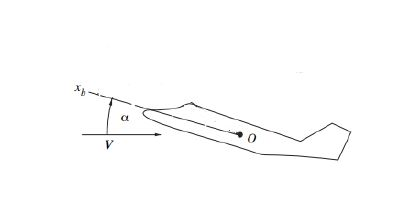
\includegraphics[width=0.6\linewidth]{Figures/Fig10}
	\caption[]Angle of attack]{Angle of attack (\textalpha) \cite{ferreira2015design}}
	\end{figure}
\end{center}
\subsection{Summary of Gaps}